

%%%%%% partie implémentation >> IaForInRow >> données de tests %%%%%%%%

 Nous devons choisir les données de tests de façon à tester l'ensemble des retours de la fonction \texttt{play(rule)}
c'est à dire :
\begin{itemize}
 \item Un entier pour la colonne dans laquelle il a jouer.
 \item Un code d'erreur si il ne peut pas jouer.
\end{itemize}

Mais aussi tester les différents états du tableau \texttt{playable[]} qui donne les stratégies comme vu ci-dessus, nous devons donc trouver des données pour obtenir les différentes valeurs possible de \texttt{playable[i]} et prouver que l'ordinateur en tiendra compte dans le choix de la position dans laquel il jouera.

Nous utiliserons donc les grilles ci-dessus avec les règles de jeux standard ( 4 pions alignés gagnent ).Nous devrons rajouter d'autres grilles comme la grille entièrement remplie pour nous assurer que l'ordinateur retourne bien un code d'erreur.Il ai envisagé d'utiliser principalement le mode difficile pour les données de test , car les deux mode ont un comportement similaire avec des stratégies supplémentaire pour le mode difficile.

%%%%%% partie tests réel ,junit...%%%%%

Nous allons donc ici tester l'ordinateur reprendre les exemples de la partie implémentation IaForInRow en ajoutant comme prévus les cas 

Les données de test se compose d'une ordinateur avec un mode (facil ou difficile) et de l'état de la structure de donnée , c'est à dire de la grille de jeux. Dans le rapport l'ensemble des tests se feront a l'aide d'une IA en mode difficile, l'IA facil ayant le même comportement avec des stratégies en moins.( certains testes sont quand même présent dans \texttt{Junit} sur l'ordinateur en mode facil et des grilles non conventionnelles )

\begin{figure}[H]
\begin{center}
  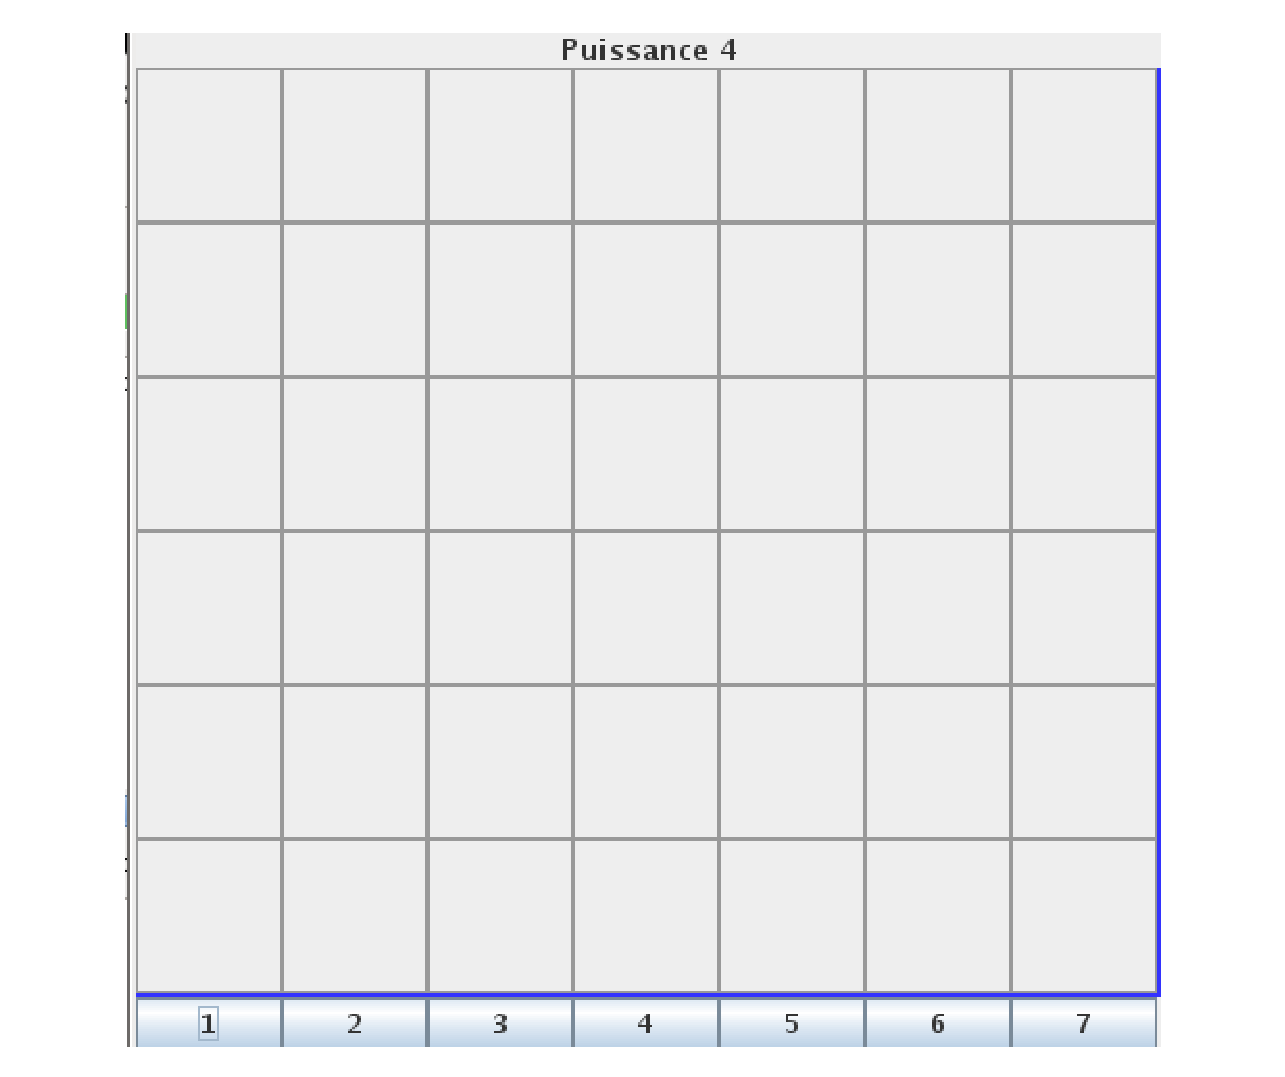
\includegraphics[scale=0.2]{nmfigempty}
  \caption{\texttt{Grille vide}}
\end{center}
\end{figure}

La grille est vide nous devons donc vérifier que l'ordinateur ne met pas encore en place de stratégie donc que 
\texttt{playable[]} est entièrement à 0 et que donc par défaut l'ordianteur joue au centre de la grille.


\begin{verbatim}
int Ia2Played = ia2.play(rule);
assertNotNull(Ia2Played);
assertTrue(0 <= Ia2Played && Ia2Played < grid.getWidth());
assertEquals(3, Ia2Played);
int[] playable2 = ia2.getPlayable();
for ( int i =0 ; i<ia2.getCpuGrid().getWidth();i++)
assertEquals(0,playable2[i]);
\end{verbatim}


\begin{figure}[H]
\begin{center}
  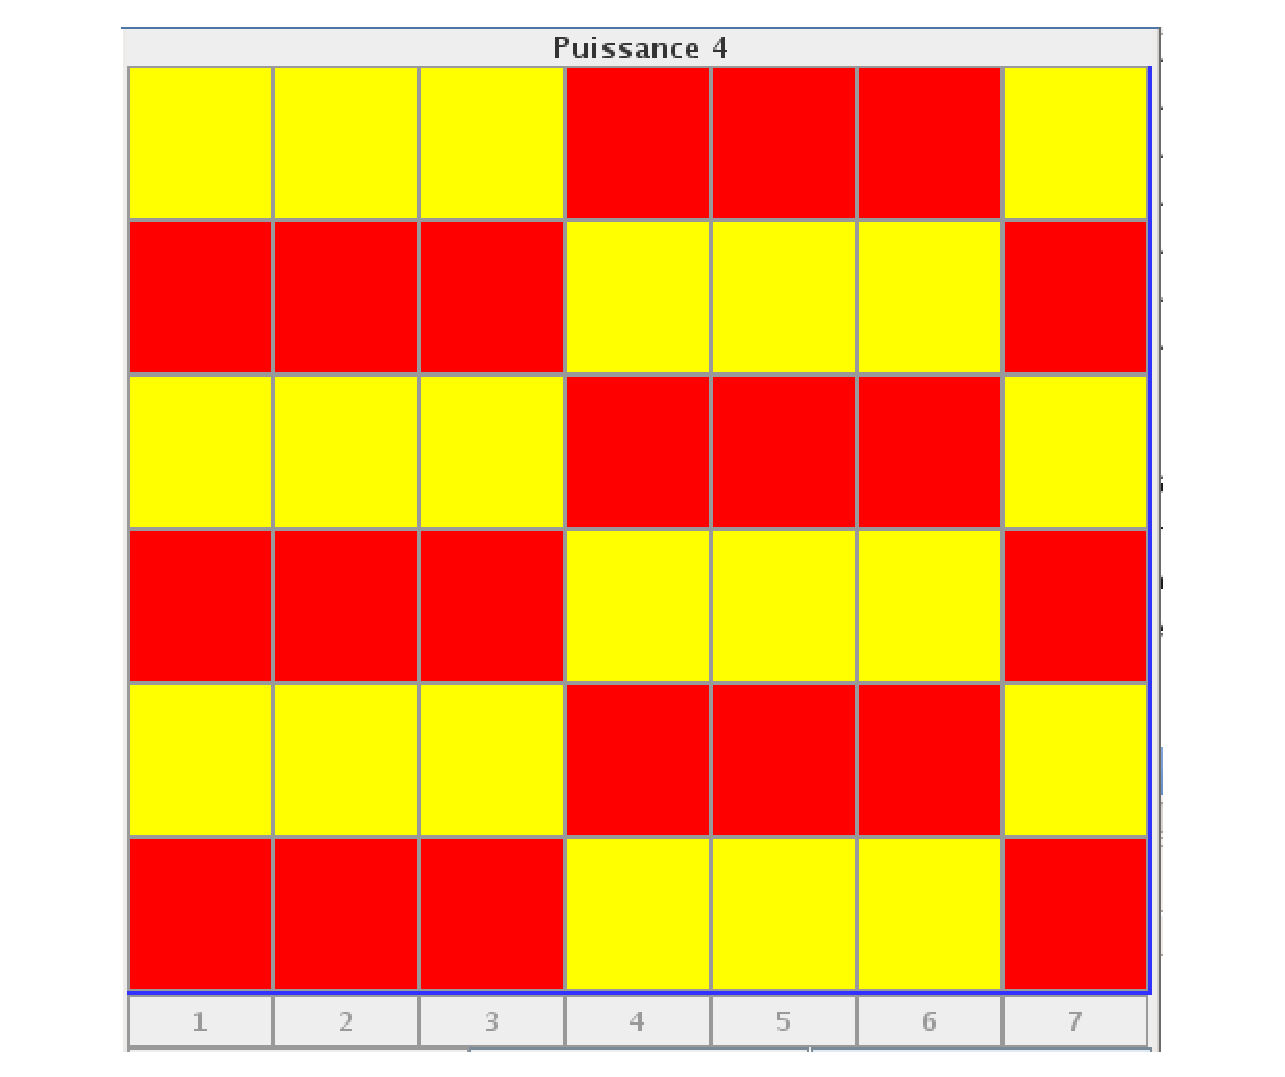
\includegraphics[scale=0.2]{nmfigfull}
  \caption{\texttt{Grille pleine}}
\end{center}
\end{figurre}

La grille étant pleine l'ordinateur ne peut donc pas jouer elle doit retrouner le code d'erreur -1.

\begin{verbatim}
 int Ia2PlayedFullGrid = ia2.play(rule);
 assertFalse(0 <= Ia2PlayedFullGrid && Ia2PlayedFullGrid < grid.getWidth());
 assertEquals(-1, Ia2PlayedFullGrid);
\end{verbatim}

\begin{figure}[H]
\begin{center}
  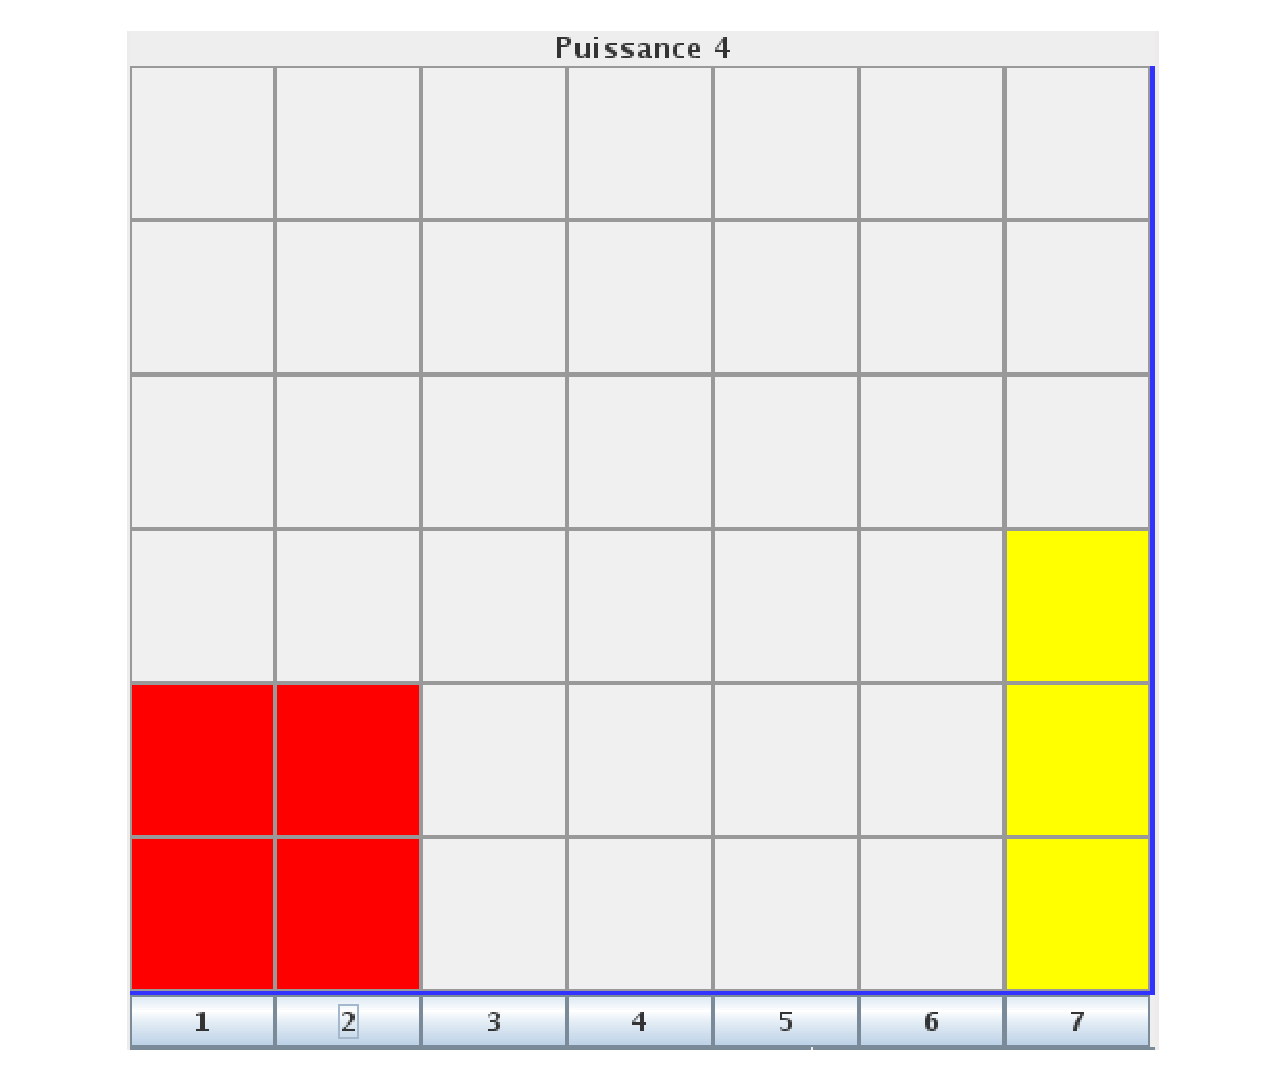
\includegraphics[scale=0.2]{nmfigwin}
  \caption{\texttt{Grille avec coup gagnant}}
\end{center}
\end{figurre}

Il y a la possibilité pour l'ordinateur de gagner elle doit donc repérer la collone qui permet de gagner en y mettant le code \texttt{playable} à 3 et y jouer.

\begin{verbatim}
 int Ia4PlayedForWin = ia4.play(rule);
assertNotNull(Ia4PlayedForWin);
assertTrue(0 <= Ia4PlayedForWin && Ia4PlayedForWin < grid_null.getWidth());
assertEquals(6, Ia4PlayedForWin);
int[] playable4 = ia4.getPlayable();
for ( int i =0 ; i<ia4.getCpuGrid().getWidth();i++)
   if ( i == 6)
assertEquals(3,playable4[i]);
   else
assertEquals(0,playable4[i]);
\end{verbatim}


\begin{figure}[H]
\begin{center}
  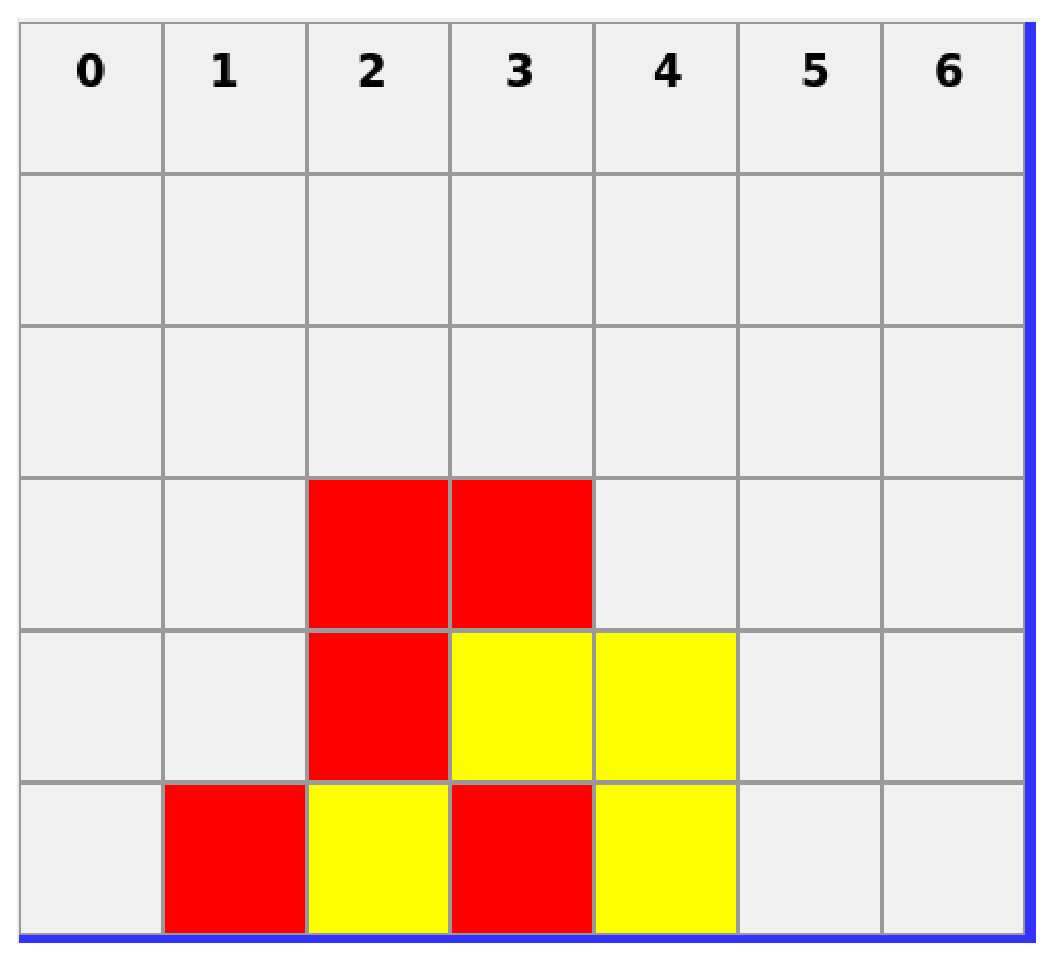
\includegraphics[scale=0.2]{playable10}
  \caption{\texttt{Colonne injouable}}
\end{center}
\end{figure}
Si l'ordinateur joue sur la colonne 4, alors au prochain coups le
joueur humain pourra gagner avec une diagonale. L'ordinateur devra donc avoir
\texttt{playable[4]=1} et jouer sur une autre case ici par la programmation nous savons qu'il va jouer en 2.

\begin{verbatim}
 int Ia2Playedfig2 = ia2.play(rule);
int[] playable5 = ia2.getPlayable();
assertEquals(2 , Ia2Playedfig2);
assertEquals(1 , playable5[4]);
\end{verbatim}


\begin{figure}[H]
\begin{center}
  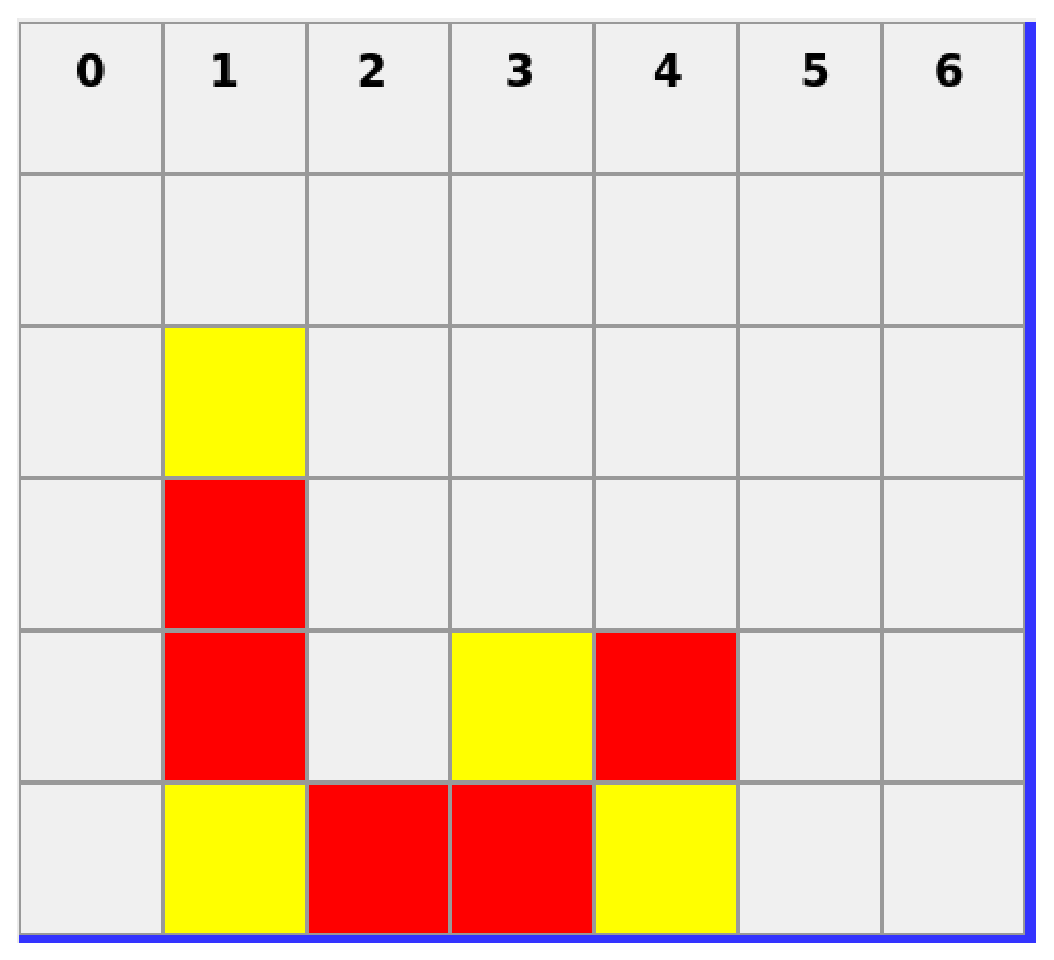
\includegraphics[scale=0.2]{playable2}
  \caption{\texttt{Strategie sur plusieur coups}}
\end{center}
\end{figure}
Si l'ordinateur joue en 2 cela permettra a l'humain de bloquer un coup gagnant 
l'ordinateur doit avoir \texttt{playable[2] = 2} ce qui est un code moins fort que 1 
mais il ne doit pas y jouer tout de même.

\begin{verbatim}
 int Ia2Playedfig3 = ia2.play(rule);
int[] playable6 = ia2.getPlayable();
assertEquals(3 , Ia2Playedfig3);
assertEquals(2, playable6[2]);
\end{verbatim}


\begin{figure}[H]
\begin{center}
  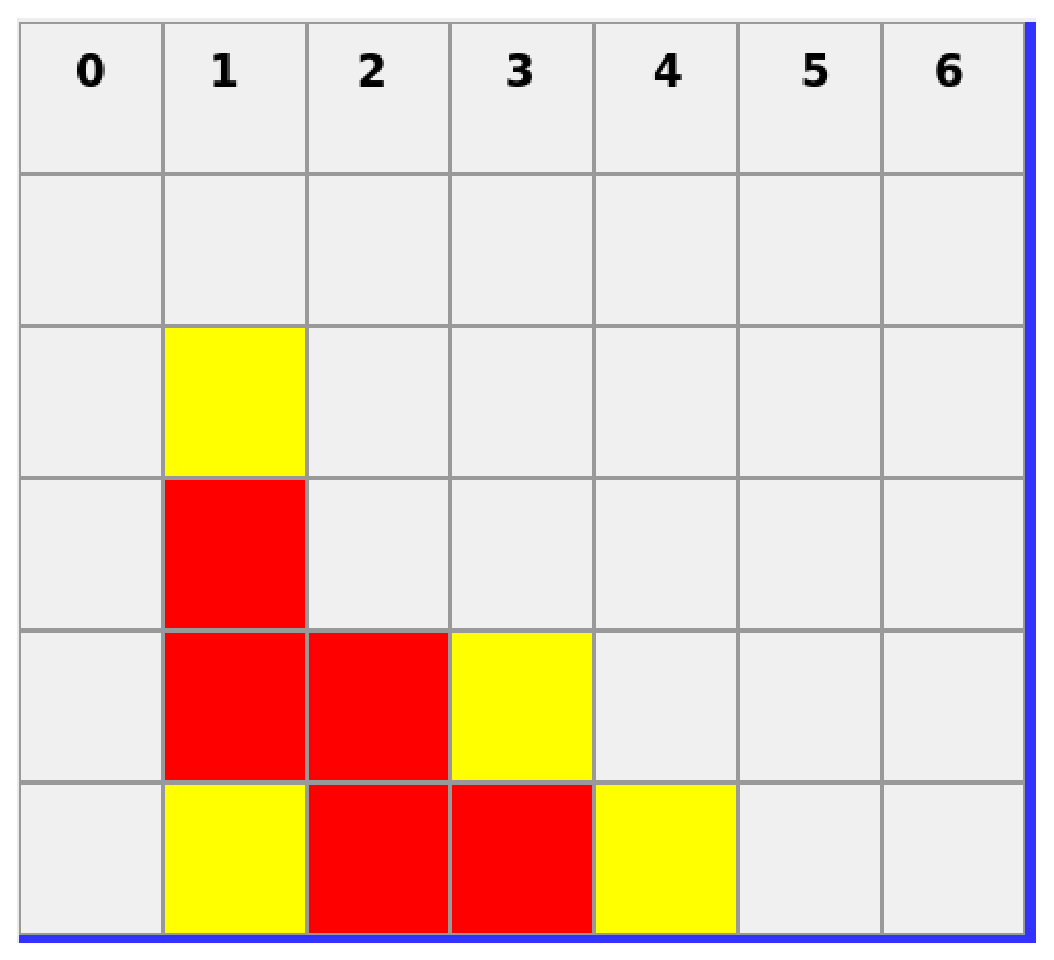
\includegraphics[scale=0.2]{playable3}
  \caption{\texttt{Autre cas de coup gagnant}}
\end{center}
\end{figure}
L'odinateur peut à nouveau gagner en jounant en jouant en 2.

\begin{verbatim}
 int Ia2Playedfig4 = ia2.play(rule);
int[] playable7 = ia2.getPlayable();
assertEquals(2 , Ia2Playedfig4);
assertEquals(3, playable7[2]);
\end{verbatim}


\begin{figure}[H]
\begin{center}
  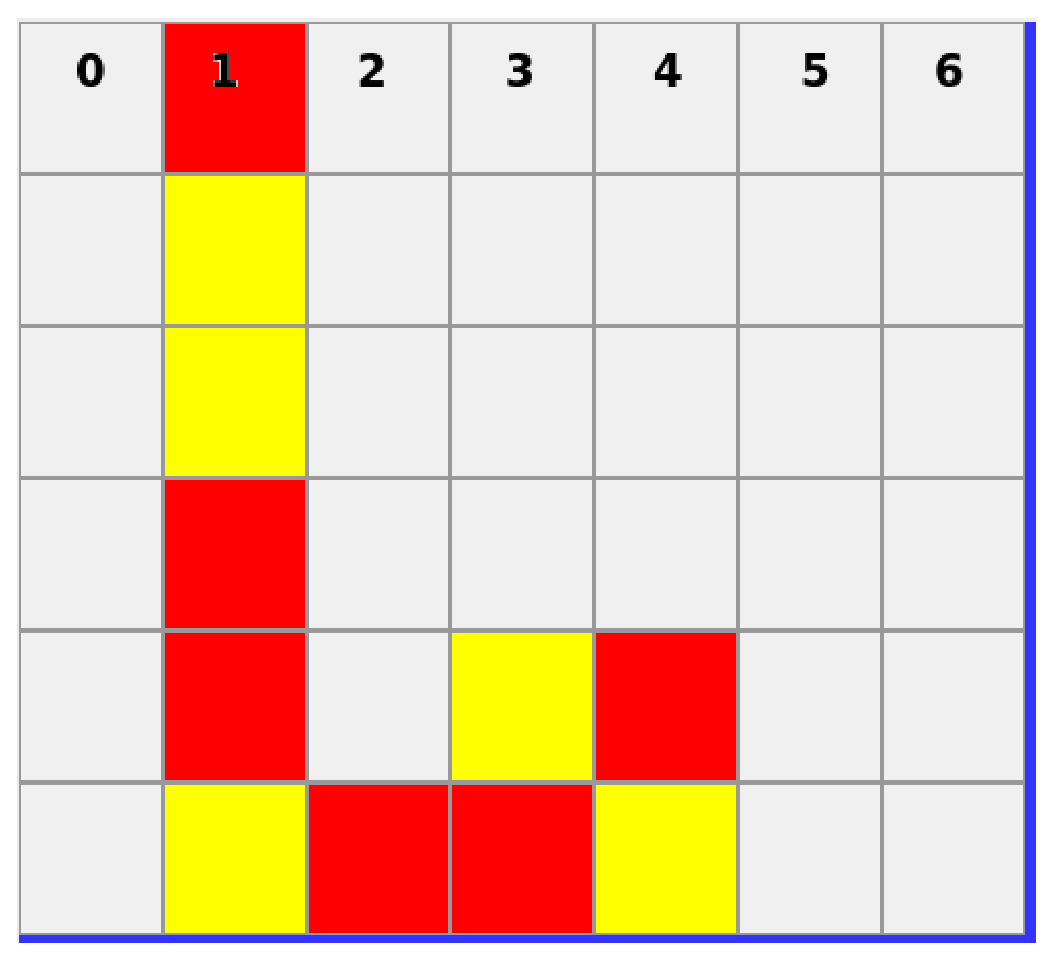
\includegraphics[scale=0.2]{playable4}
  \caption{\texttt{Colonne injouable}}
\end{center}
\end{figure}
La colonne 1 est pleine donc l'ordinateur ne doit plus y jouer et  \texttt{playable[1] = 4}.
C'est le code d'injouabilité le plus fort si tout les colonnes sont a 4 il renvera un code d'erreur -1.

\begin{verbatim}
 int[] playable8 = ia2.getPlayable();
assertEquals(4, playable8[1]);
\end{verbatim}


\begin{figure}[H]
\begin{center}
  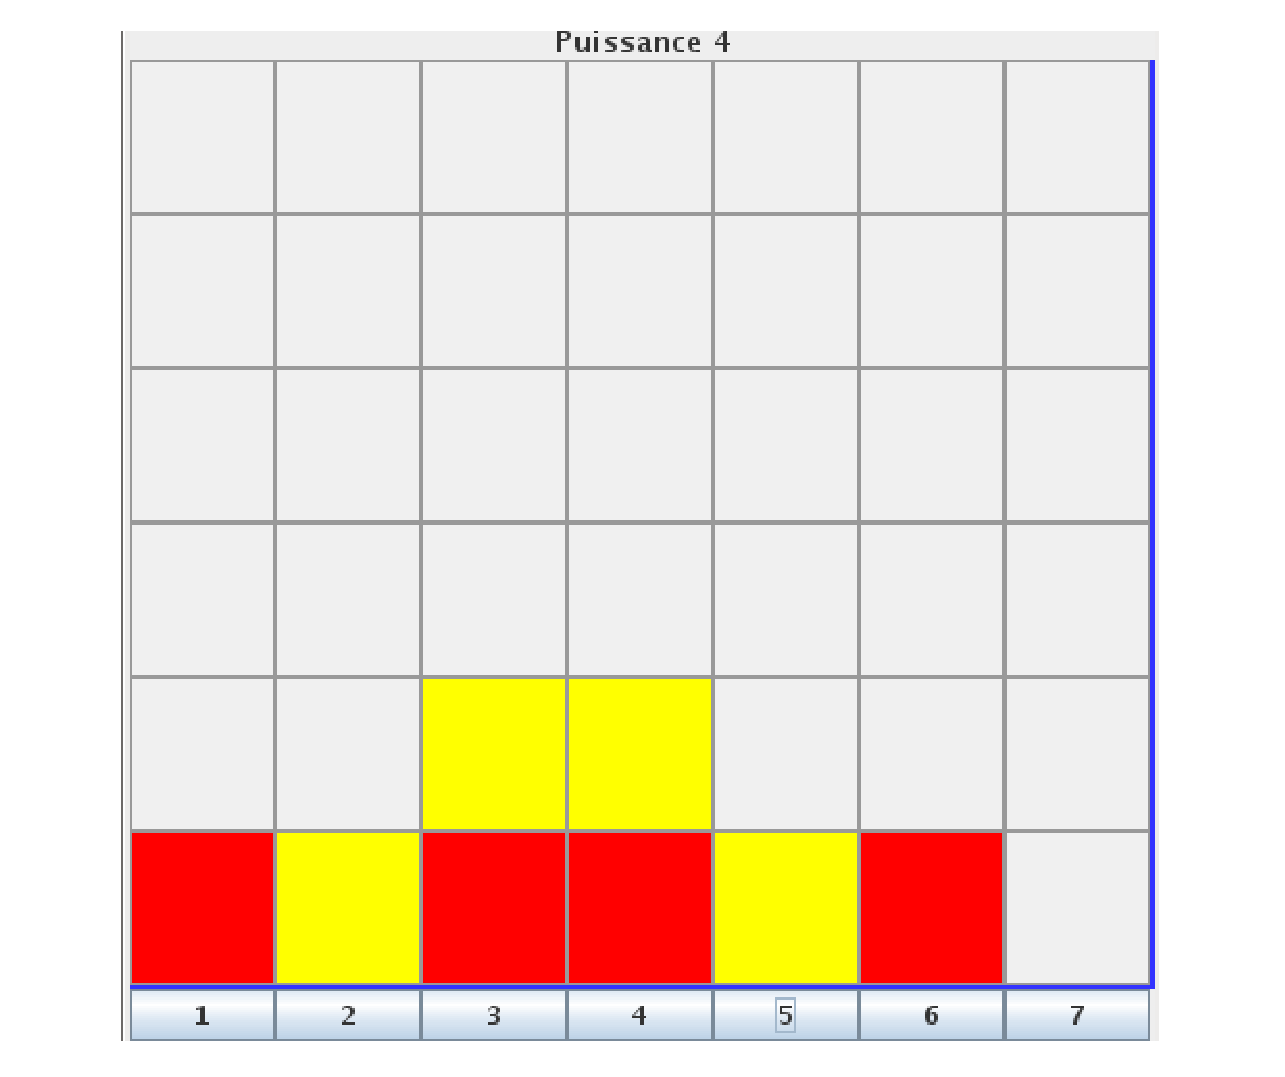
\includegraphics[scale=0.2]{nmfig6}
  \caption{\texttt{Strategie sur plusieurs coup}
\end{center}
\end{figure}
L'ordinateur doit remarquer qu'il peut gagner en deux coup il met donc \texttt{playable}
à 5 sur les cases offrant cette possibilitée : \texttt{playable[2] =  5} et \texttt{playable[5] = 5}.
(  colonne 2 et 6 sur la grille ).

\begin{verbatim}
 int Ia2Playedfig6 = ia2.play(rule);
int[] playable9 = ia2.getPlayable();
assertEquals(5 , Ia2Playedfig6);
assertEquals(5, playable9[1]);
assertEquals(5, playable9[5]);
\end{verbatim}


\begin{figure}[H]
\begin{center}
  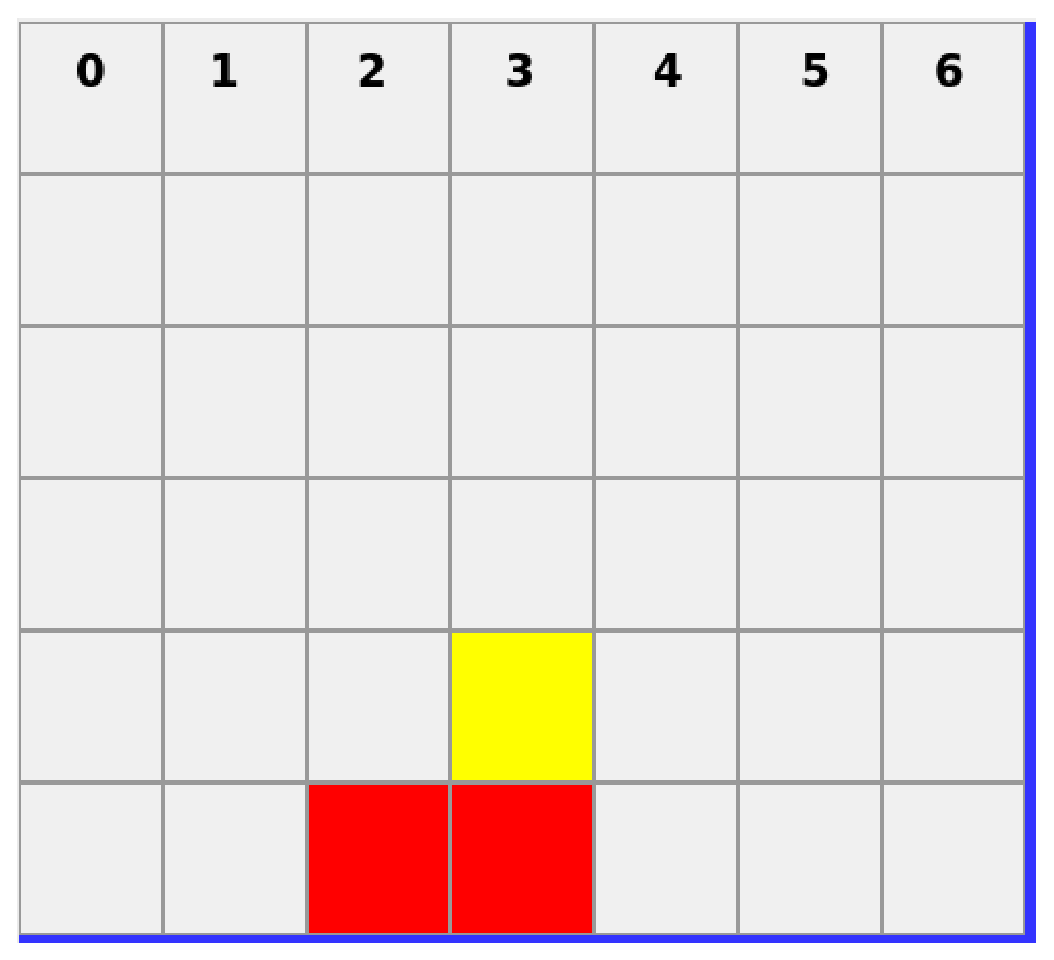
\includegraphics[scale=0.2]{playable1}
  \caption{\texttt{Strategie de bloquage}}
\end{center}
\end{figure}
L'ordinateur peut aussi prévoir à l'avance les positions dangereuses des pions de l'autre joueur,
il mettra ainsi en place la tactique \texttt{playable} 6 dans les colones qui couperont les alignements 
possibles des pions adverses.Dans ce cas la \texttt{playable[1] = 6} et \texttt{playable[4] = 6}.Il jouera donc dans
l'un de ces deux colonnes .

\begin{verbatim}
int Ia2Playedfig7 = ia2.play(rule);
int[] playable10 = ia2.getPlayable();
assertEquals(4 , Ia2Playedfig7);
assertEquals(6, playable10[0]);
assertEquals(6, playable10[4]);
\end{verbatim}


\begin{figure}[H]
\begin{center}
  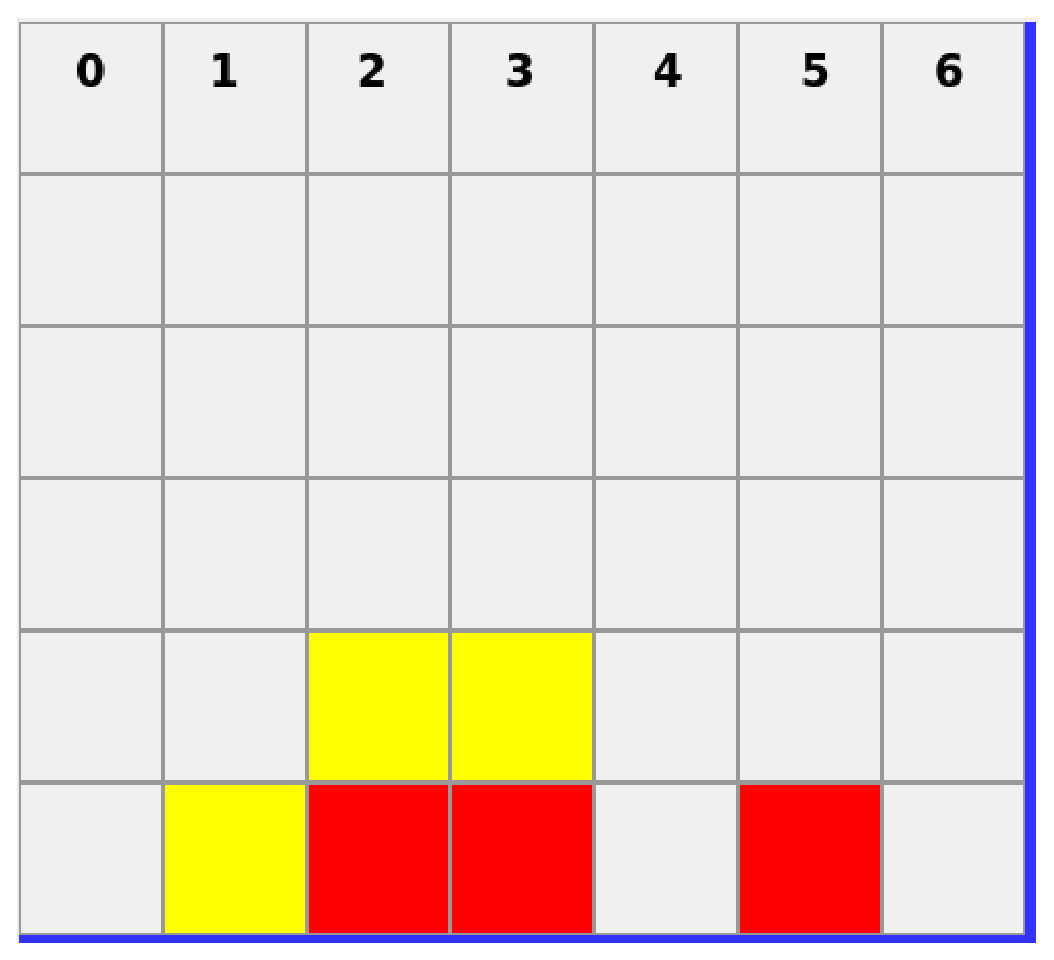
\includegraphics[scale=0.2]{playable6}
  \caption{\texttt{Coup Obligatoire}}
\end{center}
\end{figure}
L'ordinateur est obliger de jouer en colonne 4 sous peine de voir l'autre joueur gagner au prochain coup.
Nous devons donc avoir \texttt{playable[4]=6}.

\begin{verbatim}
 int Ia2Playedfig8 = ia2.play(rule);
int[] playablefig8 = ia2.getPlayable();
assertEquals(4 , Ia2Playedfig8);
assertEquals(6, playablefig8[4]);
\end{verbatim}


\begin{figure}[H]
\begin{center}
  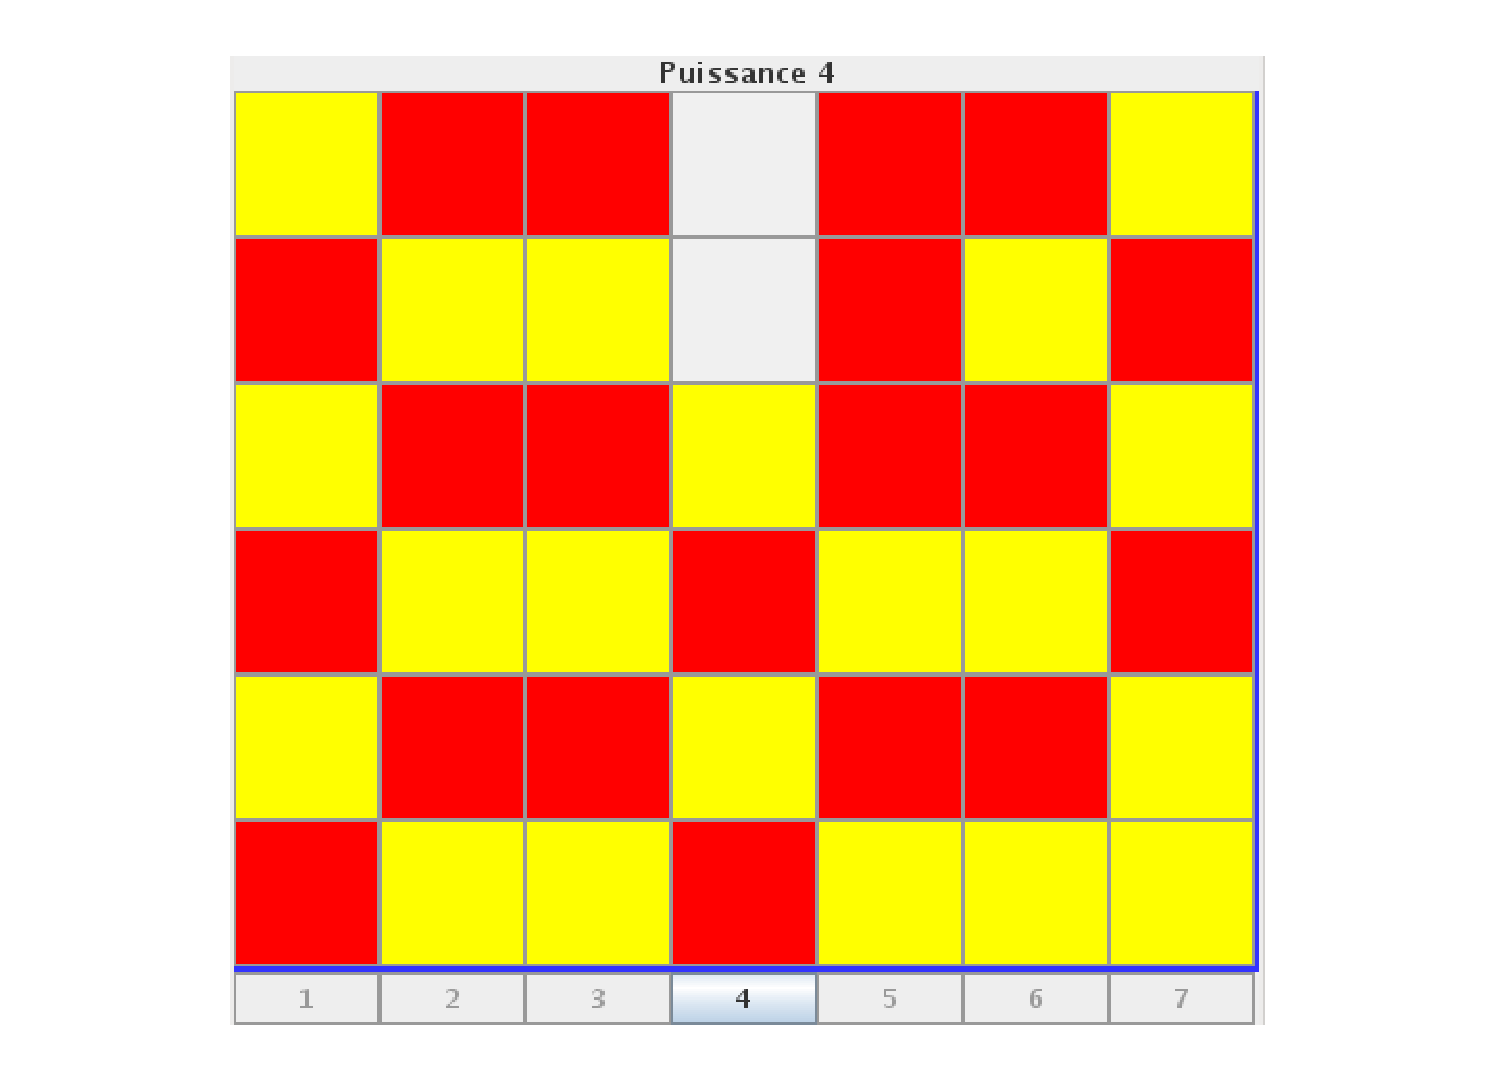
\includegraphics[scale=0.2]{nmfig9}
  \caption{\texttt{Non bloquage du jeu}}
\end{center}
\end{figure}
Il peut arriver que l'ordinateur n'est pas le choix et doix jouer dans une colonne même si son
\texttt{playble} est à 1  c'est a dire que jouer ce coup fera gagner l'autre joueur, nous devons vérifier que l'ordinateur le fera quand même sous peine de bloquer la partie.Donc ici \texttt{played[3]=1} , mais l'ordinateur joue en 3 (4eme colonne).
